

%\documentclass[journal,draftcls,onecolumn]{IEEEtran}
\documentclass[journal]{spie}
%\renewcommand{\baselinestretch}{1.65}
\usepackage[]{times}

\usepackage{subfig}
\usepackage{listings}

\usepackage[sort, numbers, super]{natbib}

\usepackage{hyperref}

\usepackage{soul}
%\usepackage[pdftex]{graphicx}
\usepackage[]{graphicx}
\usepackage{url}
   \usepackage{siunitx}

%\newcommand {\EDIT} {\ul}		% show underlined edits.
%\newcommand {\EDIT} {}		    % show underlined edits.

\usepackage{multicol}
\usepackage{amsmath}
\usepackage{overpic}

\pagestyle{plain}    
\begin{document}


\title{Schematic Driven Silicon Photonics Design \\
(Invited)}

\author{Lukas Chrostowski\supit{a}, 
Zeqin Lu\supit{a}, 
Jonas Flueckiger\supit{a},
James Pond\supit{b}, 
Jackson Klein\supit{b},
Xu Wang\supit{b},
Sarah Li\supit{a}, 
Wei Tai \supit{a}, 
En Yao Hsu\supit{a}, 
Chan Kim\supit{a}, 
John Ferguson\supit{c},
Chris Cone\supit{c}
\skiplinehalf
\supit{a}Department of Electrical and Computer Engineering, \\
University of British Columbia, Vancouver, British~Columbia, Canada \\
\supit{b}Lumerical Solutions Inc.,  Vancouver, British~Columbia, Canada \\
\supit{c}Mentor Graphics Corporation, Portland, Oregon, USA
}

\maketitle


\lstset{language=Python,
  basicstyle=\scriptsize, 
  frame=single,tabsize=2, captionpos=b,breaklines=true,showstringspaces=false,
  morecomment=[l]{\#},morestring=[b][\color{blue}]",morestring=[b][\color{blue}]'
}
\lstset{frame=shadowbox, xleftmargin=3mm, framexleftmargin=2mm, rulesepcolor=\color{blue}}
\lstset{columns=flexible}

\lstset{language=C,
  basicstyle=\scriptsize, 
  frame=single,tabsize=2, captionpos=b,breaklines=true,showstringspaces=false,
%  morecomment=[l]{\#},morestring=[b][\color{blue}]",morestring=[b][\color{blue}]'
}
\lstset{frame=shadowbox, xleftmargin=3mm, framexleftmargin=2mm, rulesepcolor=\color{blue}}
\lstset{columns=flexible}

\lstset{language=bash,
  basicstyle=\scriptsize, 
  frame=single,tabsize=2, captionpos=b,breaklines=true,showstringspaces=false,  morecomment=[l]{*},   commentstyle=\color{DarkGreen}
}
\lstset{frame=shadowbox, xleftmargin=3mm, framexleftmargin=2mm, rulesepcolor=\color{blue}}
\lstset{columns=flexible}


\lstset{language=Matlab,
frame=single,tabsize=2, captionpos=b,breaklines=true,showstringspaces=false,
%  aboveskip=3mm,
%  belowskip=3mm,
  columns=flexible,
  basicstyle={\scriptsize\ttfamily},
  numbers=none,
  numberstyle=\tiny\color{gray},
  keywordstyle=\color{blue},
  commentstyle=\color{DarkGreen},
  stringstyle=\color{Mauve},
  breakatwhitespace=true
}
\lstset{frame=shadowbox, xleftmargin=3mm, framexleftmargin=2mm, rulesepcolor=\color{blue}}
\lstset{columns=flexible}
%\lstset{basicstyle=\tiny}  % perhaps too small
\lstset{basicstyle=\scriptsize\ttfamily}  % perhaps too big?
%\lstset{basicstyle=\tiny\ttfamily}  % perhaps too big?





\begin{abstract}

Electronic circuit designers commonly start their design process with a schematic, namely an abstract representation of the physical circuit.  In integrated photonics on the other hand, it is very common for the design to begin at the physical component level.  In order to build large integrated photonic systems, it is crucial to design using a schematic-driven approach.  This includes simulations based on schematics, schematic-driven layout, layout versus schematic verification, and post-layout simulations.   This paper  describes such a design framework implemented using Mentor Graphics and Lumerical Solutions design tools.  In addition, we describe challenges in silicon photonics related to manufacturing, and how these can taken into account in simulations and how these impact circuit performance.


%This paper describes design methodologies developed for silicon photonics integrated circuits.  The approach presented is inspired by methods employed in the Electronics Design Automation (EDA) community.  This is complemented by well established photonic component design tools, compact model synthesis, and optical circuit modelling.   A generic silicon photonics design kit, as described here, is available for download at \url{http://www.siepic.ubc.ca/GSiP}.

\end{abstract}

\keywords{silicon photonics design, photonic integrated circuits design, design methodologies, electronic design automation (EDA), manufacturing variability, corner analysis}


\section{Introduction}\label{sec1}

In electronic circuit design, the complexity and scale of designs necessitated multi-user collaboration.  Namely, a team of designers with different roles, such concept and system architect, simulation expert, and layout designer, is required to implement a chip design.  In addition, there is another team, associated with the foundry that fabricates the designs, that includes device designers and process design kit developers.  The typical electronic design process begins with a schematic, namely an abstract representation of the circuit.  This requires that the foundry provides device models and layouts, embedded in a ``Process Design Kit'' (PDK) that can be used by circuit designers for their circuit simulations and to create their layout.  This partitioning of tasks is illustrated in Figure~\ref{Process_Design}.

\begin{figure}[tbp]
	\centering
	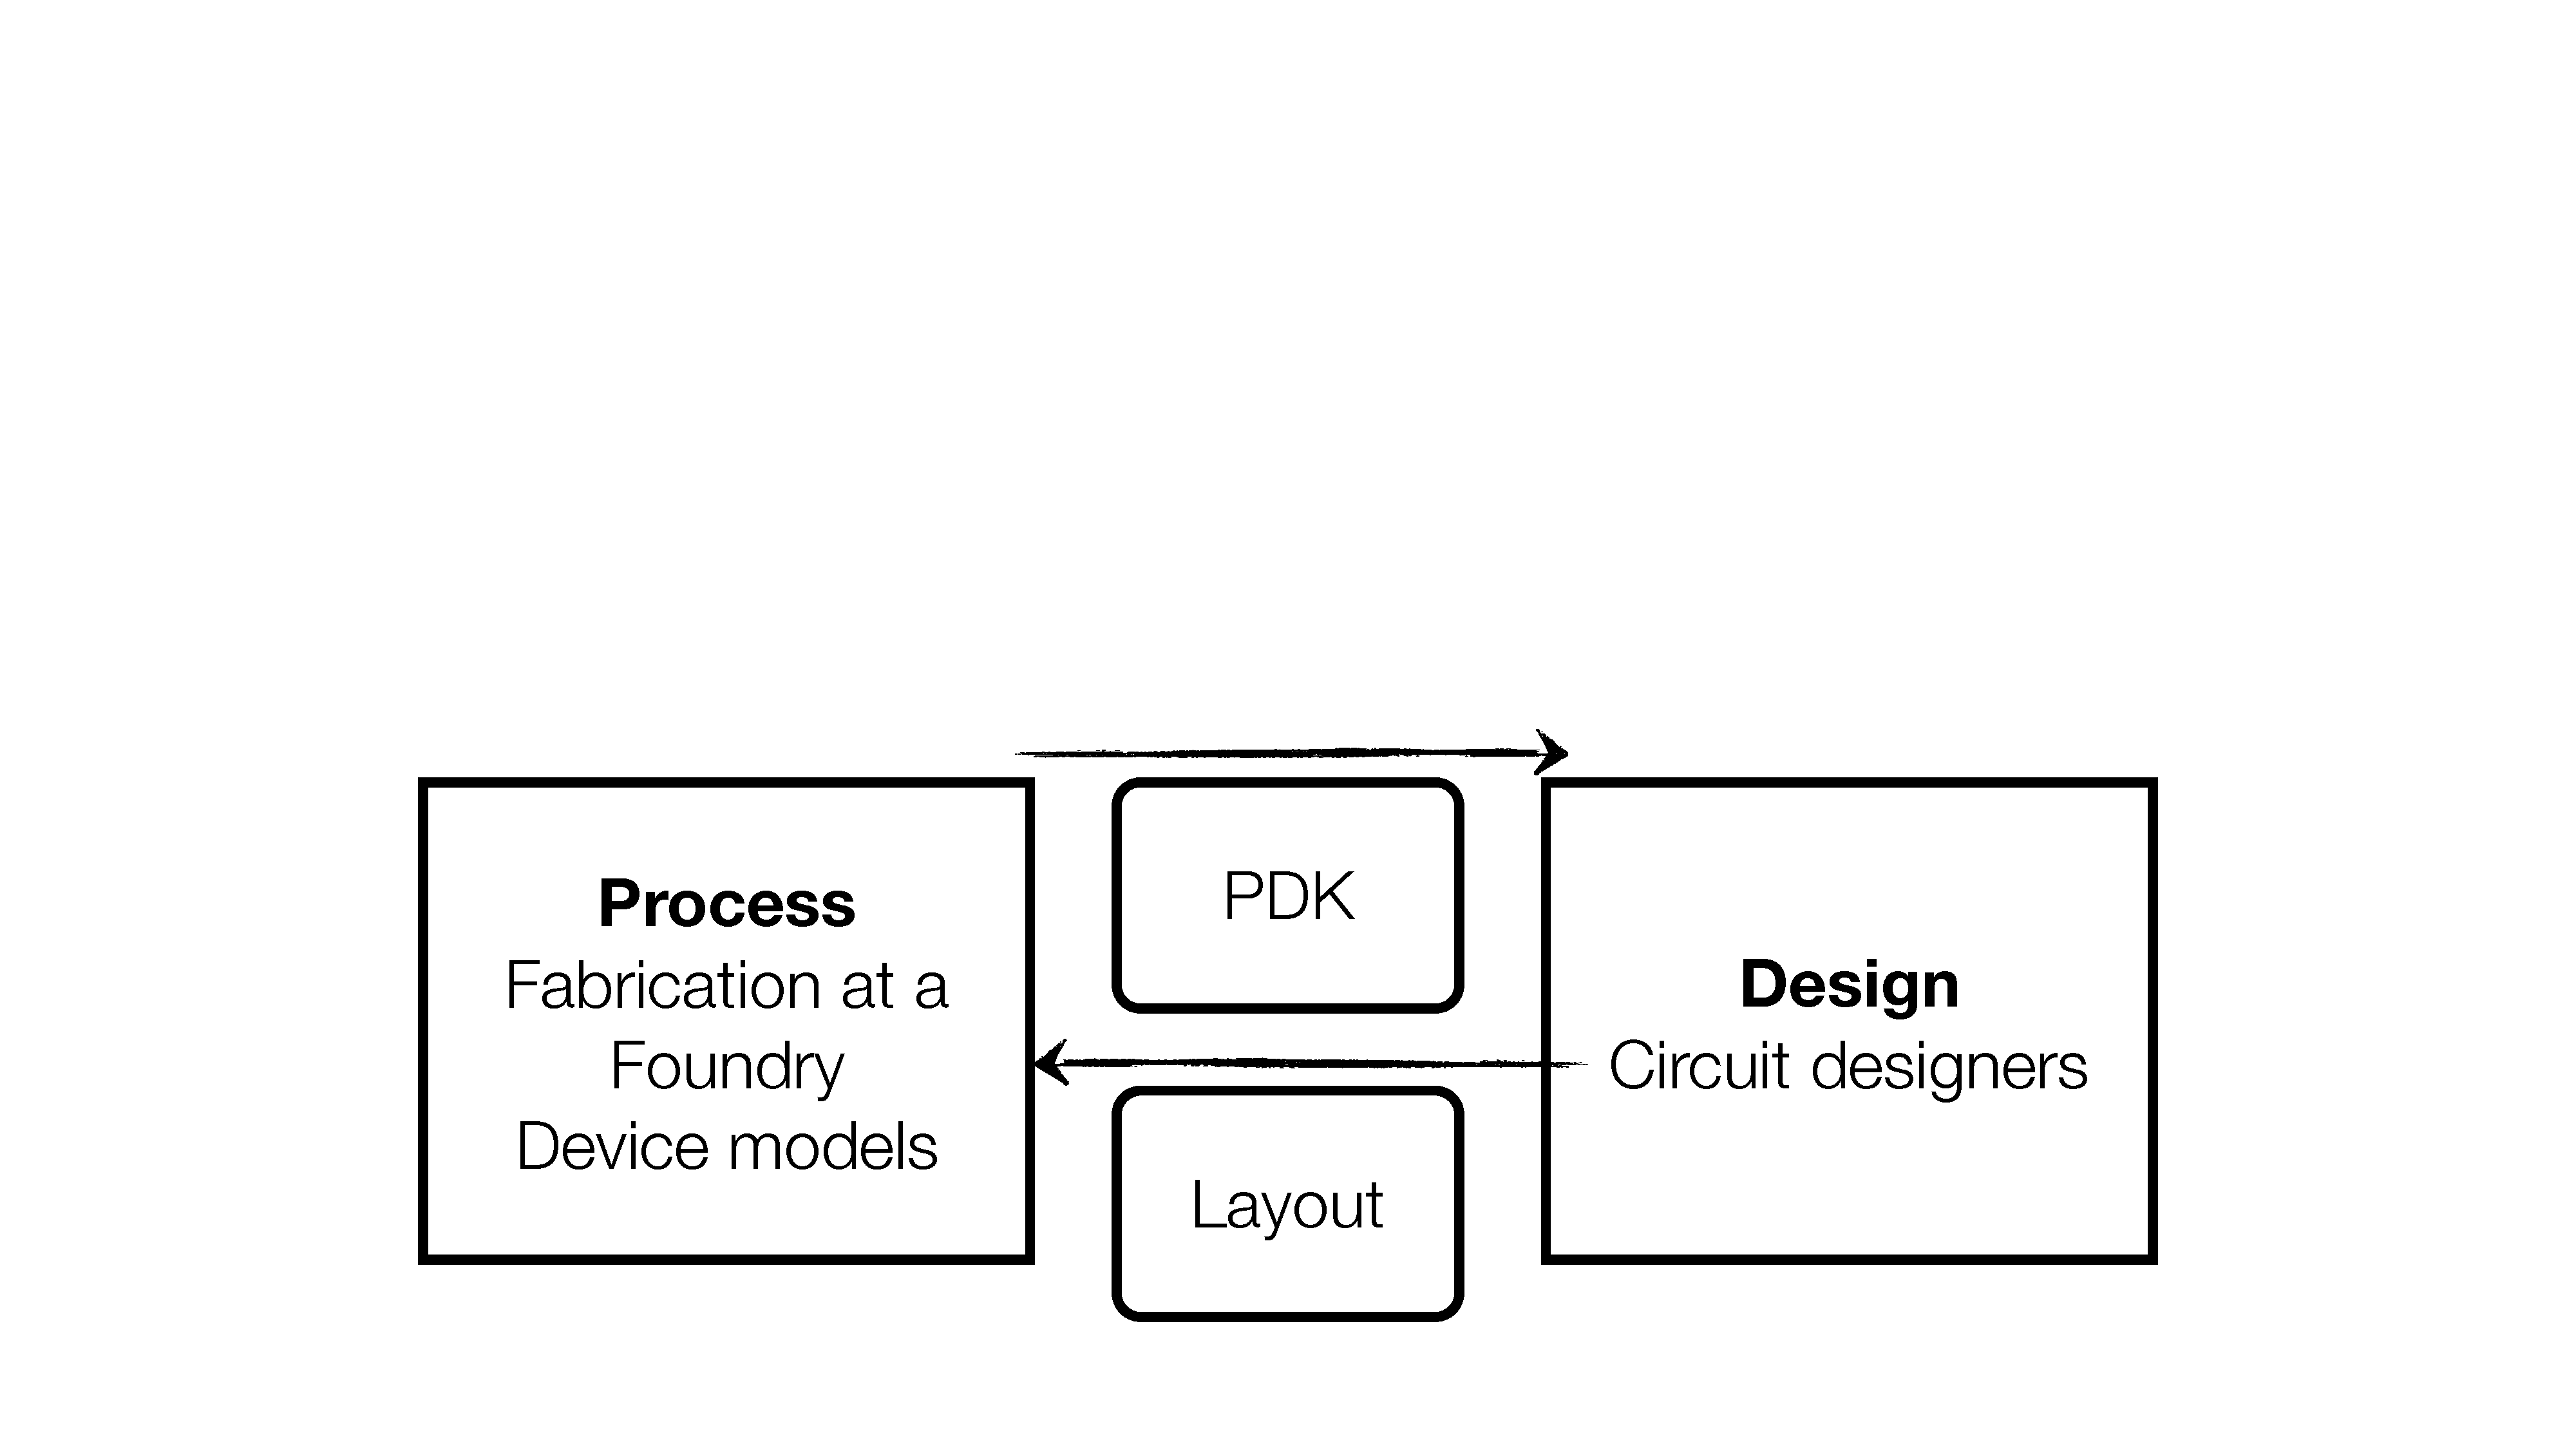
\includegraphics[width=0.5\textwidth]{../figs_paper/Process_Design.pdf}
    \caption[]{The partitioning of tasks between the foundry and the circuit designer.}
    \label{Process_Design}
\end{figure}



In integrated photonics design on the other hand, it is often one person who is responsible for all stages of the design.  Furthermore, the design process is usually ``bottom-up'', where the design begins with the physical components, and gradually builds up into a system.   In order to build large integrated photonic systems, it is crucial to 1) have a design methodology that allows for teams of designers with various roles to collaborate, and 2) have a capability that includes abstract representations (e.g., schematics) with a link to the physical implementation (layout).  

The proposed methodology is based on the electronic IC ecosystem.  This includes simulations based on schematics, schematic-driven layout, layout versus schematic verification, and post-layout simulations.   We have implemented a design framework using Mentor Graphics and Lumerical Solutions design tools that implements the above requirements, as described Refs.~\citen{chrostowski2014design, chrostowski2015silicon}.  

This paper expands upon the design methodology described previously by adding:
\begin{enumerate} 
\item Post-layout simulations
\item A choice in design style -- Schematic-Driven Design versus Layout-Driven Design
\item Manufacturing variability simulations (Monte Carlo)
\end{enumerate}
In particular, this paper emphasizes the importance of post-layout simulations.  We describe challenges in silicon photonics related to manufacturing, how manufacturing variability can be taken into account in post-layout simulations, and how these simulations can predict the impact of variability on circuit performance.

\section{Schematic-Driven Design}

First, we review the schematic-driven design approach described in Refs.~\citen{chrostowski2014design, chrostowski2015silicon}.   This design flow is aimed at highly-complex silicon photonic circuits, analogous to how they are designed in the electronics industry.  Here, the design flow starts with an abstract representation, i.e., a circuit schematic.  We begin with symbols for the components,  place them on a schematic, and connect them.   This allows us immediately simulate the circuit by providing the desired stimulus.  Behind the scenes, there are component models.  The designer does not need to develop them, since they are provided in the design kit.  Advanced PDKs will include active optical components, and electronics.  

In this flow, the layout is created on the basis of the schematic.  The software aids the designer in creating the layout by reading the schematic as the layout is generated; specifically component placement can be inferred from the schematic, and the connectivity between components is maintained to aid in the routing.

The verification step involves two parts: 1) manufacturing verification (minimum features size, etc), known as Design Rule Check (DRC), and 2) functional verification, known as Layout Versus Schematic  (LVS).  The latter is critical for large circuits.  Since we have a schematic and a layout, we have the opportunity to compare them.  The LVS tool uses a set of rules to recognize the components and their connectivity in the layout, known as netlist extraction, and then compares the components and connectivity with the original schematic.  This verification step can identify incorrect connectivity, such as disconnected wires and waveguides, and component errors such as incorrect components or incorrect parameters.

Once the layout of the circuit is deemed to be correct, the LVS tool can extract the parameters from the layout and update the schematic.  For photonics, the lengths of your waveguides, as drawn, is often critical in determining the performance.  For example, the lengths of the waveguides in an interferometer need to be calculated so that we can obtain an accurate estimation and simulation of the free spectral range (FSR). After the schematic is updated, the designer can re-simulate the circuit to verify that it operates as expected once the details (such as waveguide length in photonics, or parasitics in electronics) are included.


In contrast to the traditional photonics design approach, this design flow has a much more well established design kit, and enables rapid design of complex circuits, without having to spend time on modelling individual components.  This type of design has been critical to the success of the electronics industry where circuits have thousands to billions of components.

An evolution that is expected for integrated photonics design is that we are moving towards a methodology similar to CMOS design leading to a distinct skill sets.  For example, circuit designers will need to know the minimum of information about how a directional coupler works, but will not need to design them. For example, the main knowledge required is that it's function is similar to a beam splitter.  However, the circuit designer will be highly attune to the performance criteria of the splitter (e.g., wavelength dependance of the splitting ratio, insertion loss, power splitting balance, sensitivity to manufacturing variations) and how these impact the circuit performance (e.g., extinction ratio, crosstalk).  This enables the circuit designer to focus on design at a higher level, including system implementation.


\subsection{Post-Layout Simulation}

Post-layout simulation refers to circuit simulations that are performed after the layout is created.  In the schematic-driven design flow, this involves extracting parameters from the layout, and updating the schematic.  However, this is another use case for post-layout simulations.  Namely, we desire the capability to simulate directly from a layout without requiring a schematic (e.g., created by a different designer,  created using different software, and in general if the schematic is not available).

In this case, the LVS tool can be used to create a netlist representation of the circuit.  This is in fact easier to perform than the layout versus schematic operation described above, as it only requires the netlist extraction step.  The requirement for this functionality is that each component is supported by the library / PDK.  This is necessary so that the LVS tool can recognize the devices correctly, and label them with the appropriate component model.  Typically, the components have added marking layers that identify the components, perhaps their names, where the input / output ports are, and provide port names.

After the layout extraction done, the circuit simulator tool is used as before to perform simulations, based on the netlist.

\section{Layout-Driven Design}

The capabilities developed for post-layout simulation allow us to consider another design methodology, namely layout-driven design.   This second approach begins with the layout, as shown in Figure~\ref{SDDvsLDD}.  First the designer creates a layout, then simulates it directly from the layout.  The simulation is performed by two steps: a) netlist extraction and b) circuit simulations.  

This approach may be appealing to traditional photonics designers who have independent design stages: device modelling, circuit design, and layout.  In this traditional flow, there is no communication between these stages, hence verification and post-layout simulation is challenging.  In the case of separate tools, the need for schematics may not even be obvious or required.  For these designers, the benefit of including post-layout simulations in the layout-driven design flow is that accurate simulations can be generated based on the design.  An inspection of the simulation results, and comparison with expectations, is an excellent verification step.

Another advantage of the layout-first approach is that it provides insight into what is physically realistic, prior to doing abstract circuit design in a schematic.  For example, creating a layout first gives the designer insight into how large the library components are, how long the waveguides will need to be, how far apart the components will need to be, how many waveguide crossings will be required, etc.  

Another design option is to create a draft layout with arbitrary component parameters and use the post-layout simulation functionality to create the files necessary circuit modelling.  Once the project is setup with all components and stimulus found in the layout, the designer can proceed to optimize the design within the circuit modelling tool.  For example, in a WDM ring modulator transceiver, the choice in ring resonator parameters can be performed in the circuit modelling tool, using the realistic simulation environment created from the layout extraction tool.  In such a design flow, it is also important to have the capability for the component parameters to be synchronized between the circuit simulation and the physical layout.

Clearly, there are several design flows that are enabled by the capability of extracting the netlist from the physical layout.  The layout-driven design approach is likely to be attractive for small circuit designs.

%The first is the way it is done in electronics.  We start with a schematic, then simulate it, create a layout, and simulate again. That?s how analog electronics design is done.

Both of these design flows (schematic-driven and layout-driven) require that there is a connection between the layout and the schematic, and in both directions.  Both need a library of components, containing component models, component layouts, and component layout recognition rules (called an LVS rule deck).  The biggest challenge for the designer is to obtain access to all the necessary pieces, namely to have access to a state-of-the art PDK similar to those available in the electronics industry.  


\begin{figure}[tbp]
	\centering
	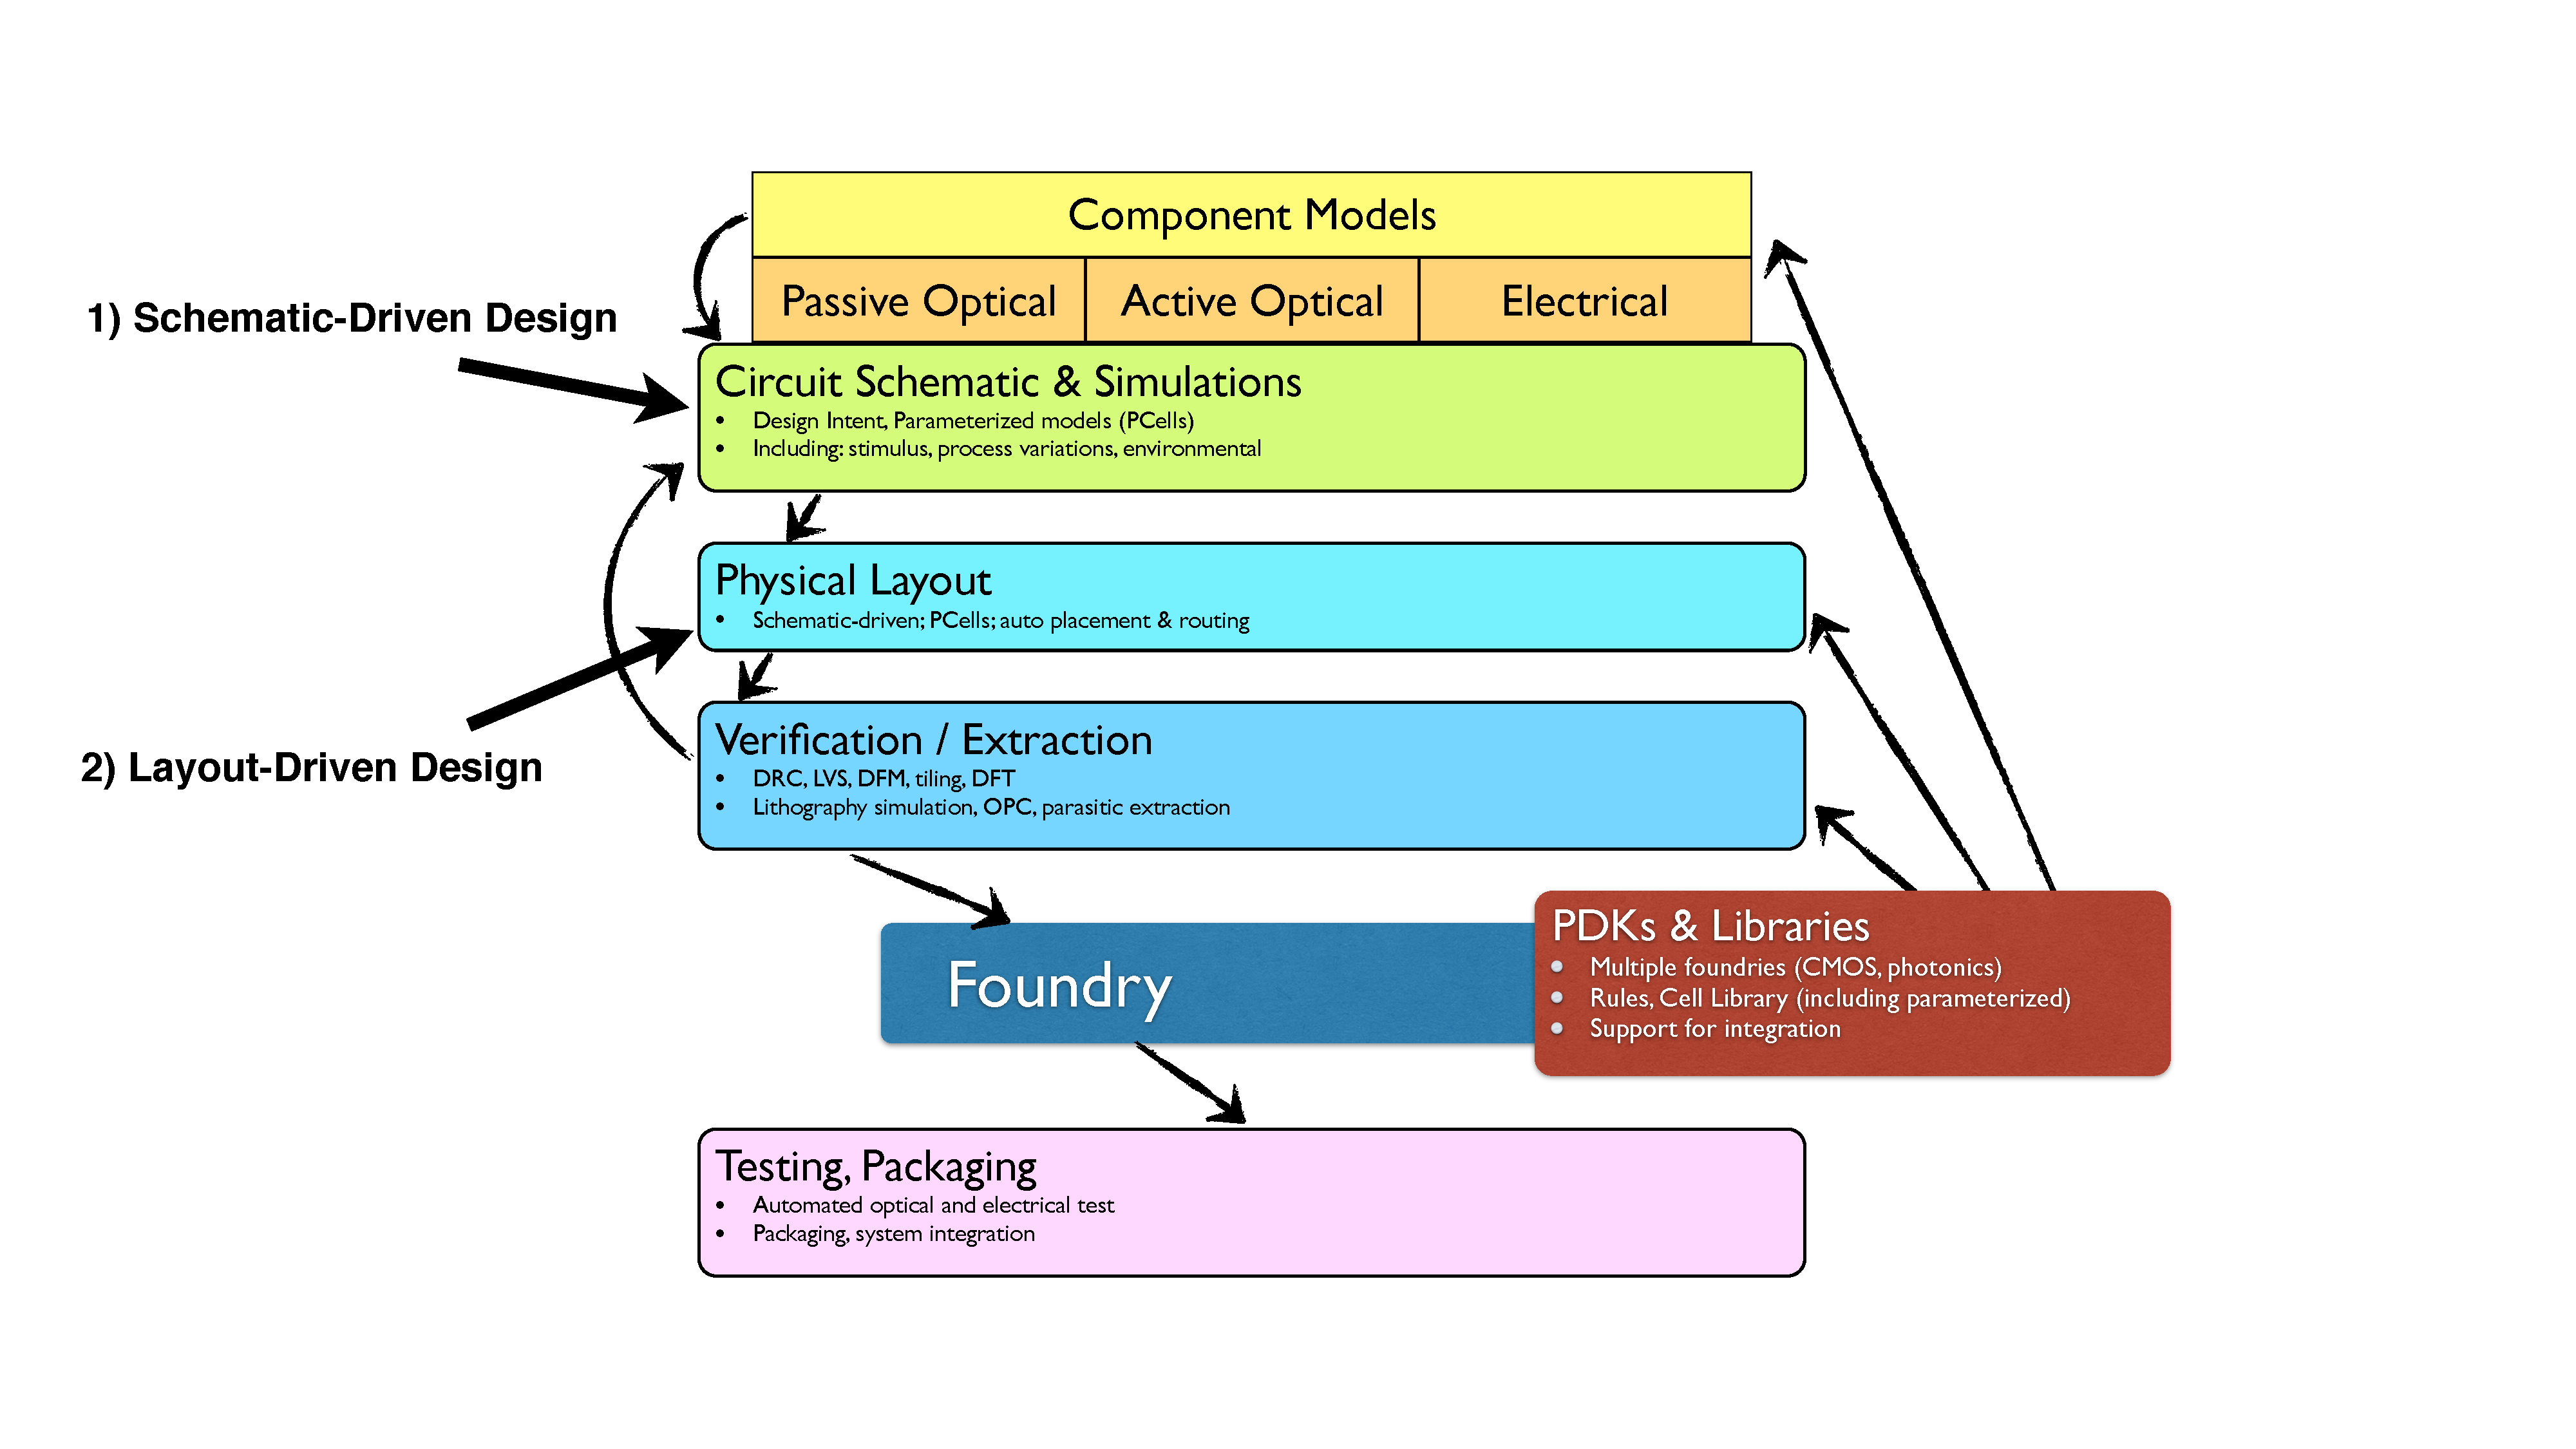
\includegraphics[width=0.9\textwidth]{../figs_paper/SDDvsLDD.pdf}
    \caption[]{Design methodology based either on 1) Schematic-Driven Design, or 2) Layout-Driven Design.}
    \label{SDDvsLDD}
\end{figure}


\section{Layout Extraction}

In this section, we provide further details on the layout extraction and netlist generation procedure.  
As discussed above, extracting the netlist from the layout is important for two reasons: 1) to verify the layout, with respect to the abstract (schematic) representation, 2) to simulate the as-drawn layout, which will include the precise waveguide lengths and component position information.  The post-layout simulation is an important verification step to ensure that no errors were introduced during the layout (e.g., disconnected waveguides leading to back-reflections).

In this section, we describe an example layout -- a Mach-Zehnder Interferometer circuit as shown in Figure~\ref{MZI_circuit2}.  It consists of two fibre grating couplers, two broad-band splitters \cite{lu2015broadband}, and numerous waveguides and waveguide bends.  The netlist is extracted from the layout, either using Mentor Graphics Calibre Layout Versus Schematic (LVS), or using the open-source KLayout \cite{www_klayout} tool with the SiEPIC-EBeam-PDK add-on \cite{siepic-ebeam-pdk}.  The extracted netlist is shown in Listing~\ref{MZI_circuit2.spi}.  Although this is a simple circuit, the listing is quite long and involves 18 components.  
Each component includes the following information:
\begin{itemize}
\item The nets to which each component pin is connected to (e.g., N\$2)
\item The library which contains the component's compact model to be used for simulations (e.g., ``Design kits/ebeam\_v1.2'')
\item The component position in the layout (lay\_x, lay\_y)
\item Optionally, a position for the component to be used in drawing the schematic (sch\_x, sch\_y)
\item Component parameters, for components that are parameterized.  For the waveguides, the parameters are the waveguide width and length.    For bends, the parameters are the radius and the waveguide width.
\end{itemize}

In the above circuit, the waveguide is broken up into straight sections and waveguide bends.  The advantage of separately listing these components is that it allows the circuit simulation to be as detailed as possible.  For example, the circuit simulation can include:
\begin{itemize}
\item An accurate model for the waveguide bend, including the insertion loss, the optical phase through the device, and the reflections from the mode-mismatch from the straight-to-bend region.
\item Position information for all these components can be used for thermal modelling and for Monte Carlo simulations, as described below.
\end{itemize}
Such an approach is particularly useful if the designer has a choice of waveguide bend radius, and the impact of the bends is not known a priori.  A simulation with that includes numerous waveguide bends with a too-small bend radius would predict the Fabry-Perot cavities introduced by the small reflections at all interfaces.  

However, in many cases, the bend has already been optimized, analyzed and chosen so that it has little impact on the circuit performance.  In that case, precise knowledge of the bend location is not necessary to include in the circuit model, nor is the bend itself.  An alternative representation of the above circuit is one where the waveguides and bends are merged into a single waveguide object.  This approach reduces the size of the netlist, and improves on the performance of the circuit simulations.  One modification is made to the waveguide object as follows:
\begin{itemize}
\item The waveguide length includes the straight sections, and the waveguide bends.  The length of the waveguide bends is taken as $L = \pi r/2$, where $r$ is the radius taken at the centre of the waveguide.
\item The waveguide has an additional parameter, namely a vector of points, e.g., points=``((-59050, 5000), (-45690, 5000), (-45690, -117300), (-59050, -117300))''  [units of nanometers].  These are used in the Monte Carlo analysis described below.
\end{itemize}



\begin{figure}[tbp]
	\centering
	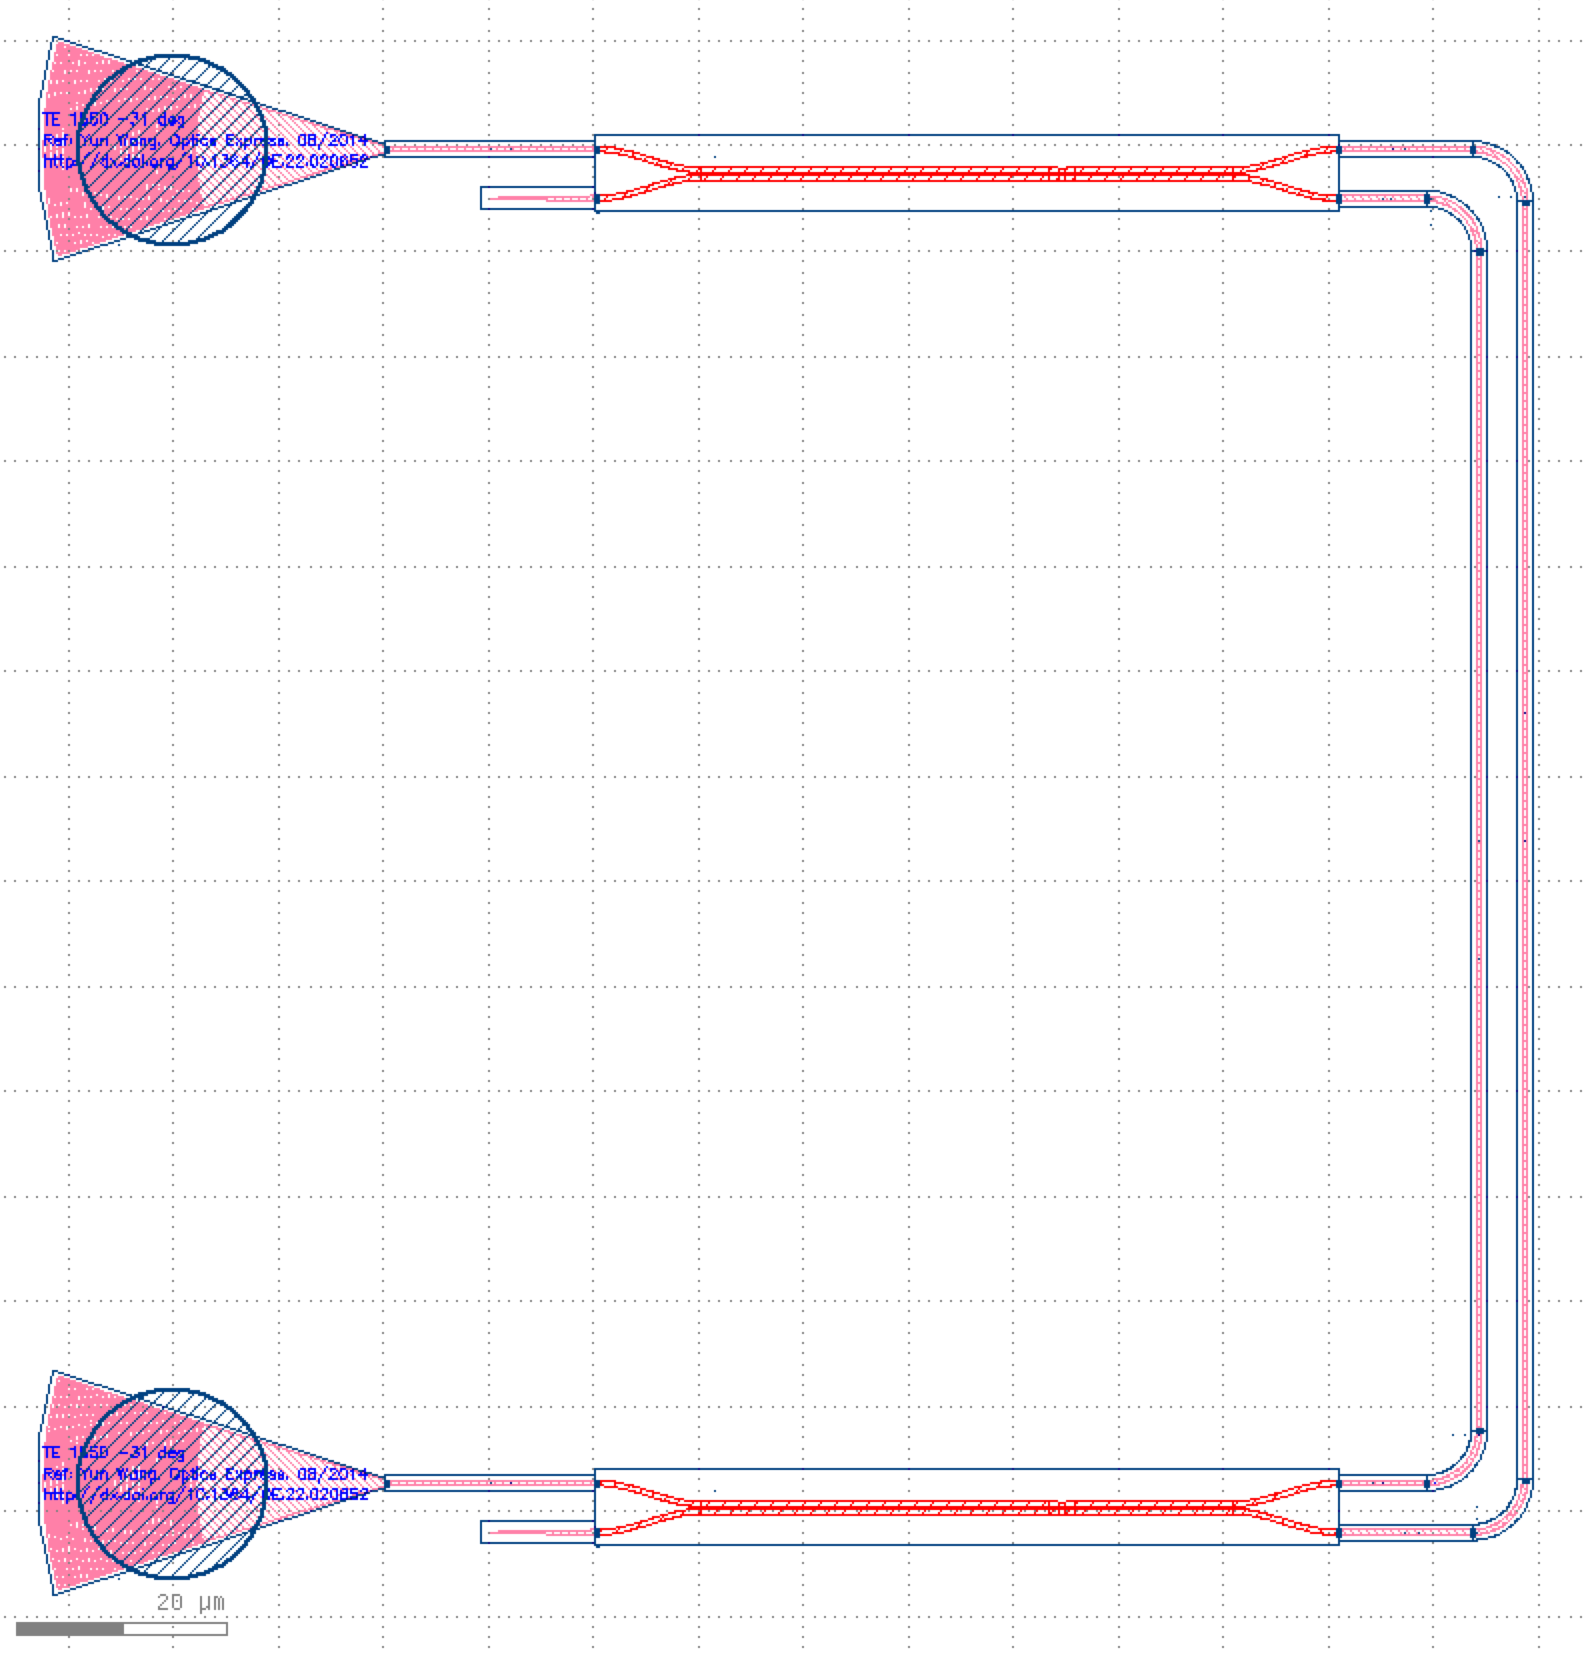
\includegraphics[width=0.5\textwidth]{../figs_paper/MZI_circuit2.png}
    \caption[]{Example layout of a Mach-Zehnder Interferometer circuit.}
    \label{MZI_circuit2}
\end{figure}

\lstinputlisting[language=Python, caption={Netlist, in SPICE format, for a Mach-Zehnder Interferometer circuit. This netlist includes all bends as separate components.},label=MZI_circuit2.spi]{MZI_circuit2.spi}

\lstinputlisting[language=Python, caption={Netlist, in SPICE format, for a Mach-Zehnder Interferometer circuit. This is a simplified netlist where the waveguides and bends are grouped into a single waveguide object.},label=MZI_circuit3.spi]{MZI_circuit3.spi}




\section{Circuit Simulations}

We previously described how to perform circuit simulations of photonic circuits using compact models created from S-parameters \cite{chrostowski2014design, chrostowski2015silicon}.  This is a powerful technique since it allows any passive device to be represented, without having to establish expressions that describe the behaviour of the component.  Efficient circuit simulations can be by achieved by using S-parameters directly, in particular for frequency (wavelength) domain simulations, as the S-parameters are already wavelength dependant.  For time domain simulations, the circuit modelling tool internally converts the S-parameters into a time-domain representation.  

We provide an example of a Bragg grating cavity test structure layout in Figure~\ref{Bragg}, together with the simulations from the extracted netlist.  The response of the circuit deviates from the ideal Bragg grating cavity response, due: 1) the grating coupler insertion loss, 2) the back-reflections from the grating couplers, and 3) the insertion loss and back-reflections from the tapers.  Ripples are observed in both the transmission and reflection spectra, that are not present in the ideal model.  Furthermore, the shapes,  positions, and oscillation frequencies of the ripples are dependant on the optical phases introduced by the various components, such as the waveguides.  Hence it is important to extract the lengths and device parameters for an accurate simulation.

\begin{figure}[tbp]
\begin{center}   
\subfloat[Layout of a Bragg grating cavity test structure.]{\label{Bragg1} 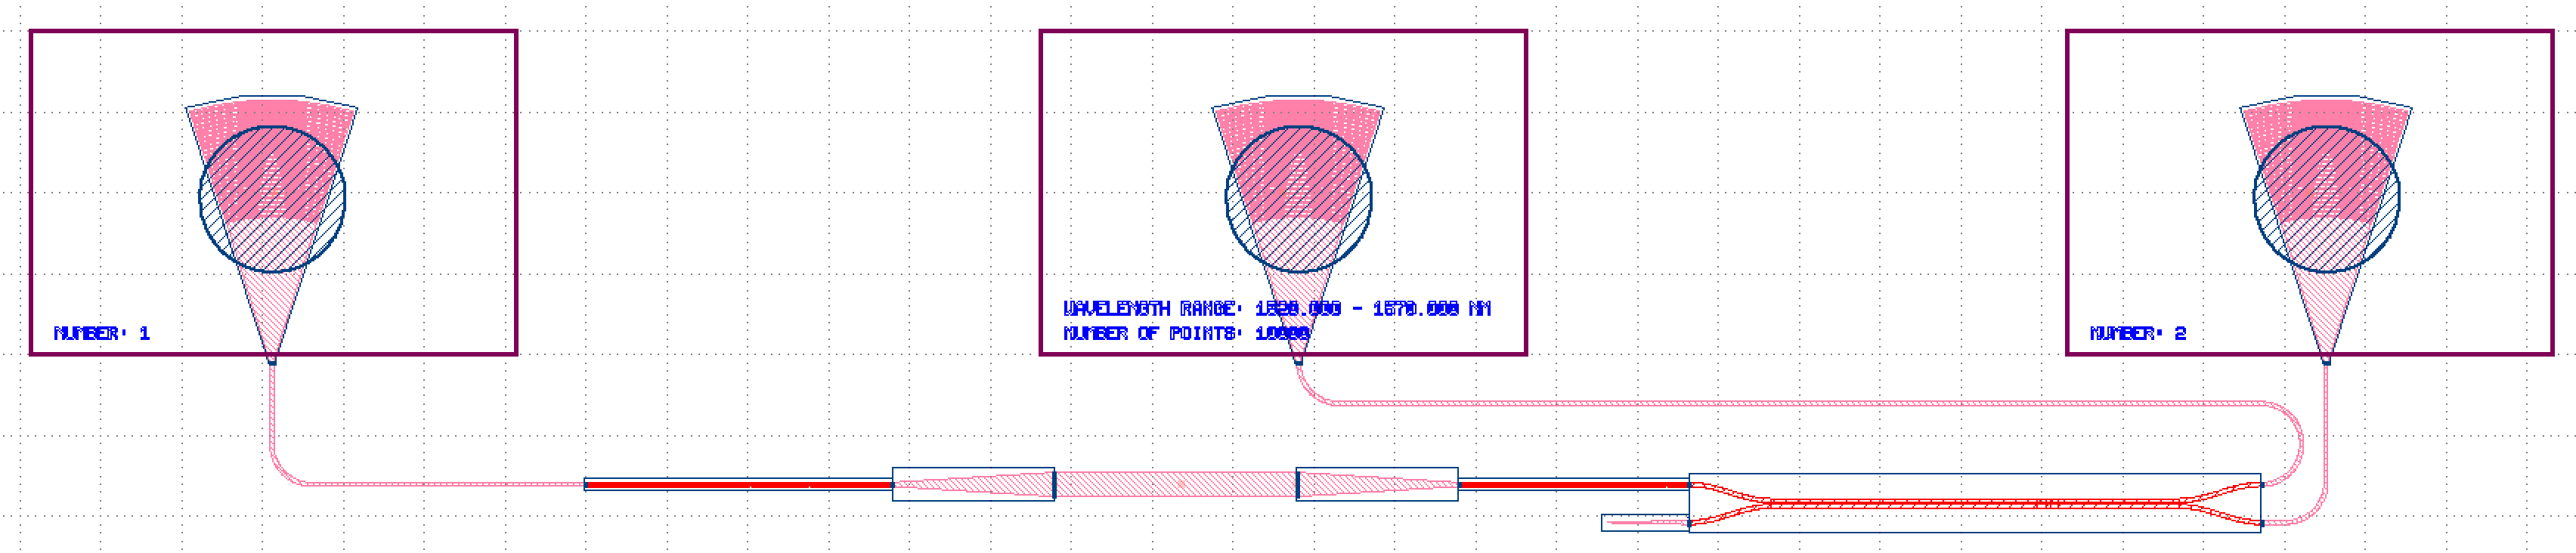
\includegraphics[width=0.8\linewidth]{../figs_paper/Bragg1} } \\
\subfloat[Zoom of the Bragg cavity, showing a portion of the Bragg grating and the taper.] {\label{Bragg2}
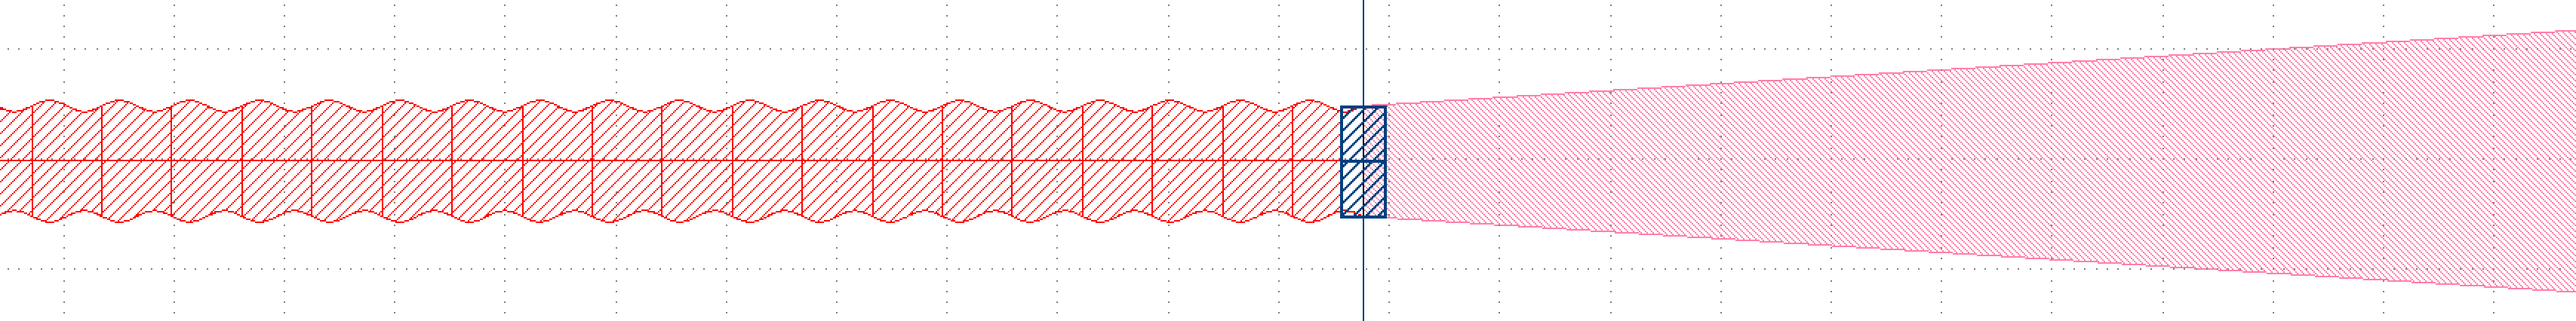
\includegraphics[width=0.8\linewidth]{../figs_paper/Bragg2} } \\
\subfloat[Circuit simulation of the Bragg grating test structure.] {\label{Bragg}
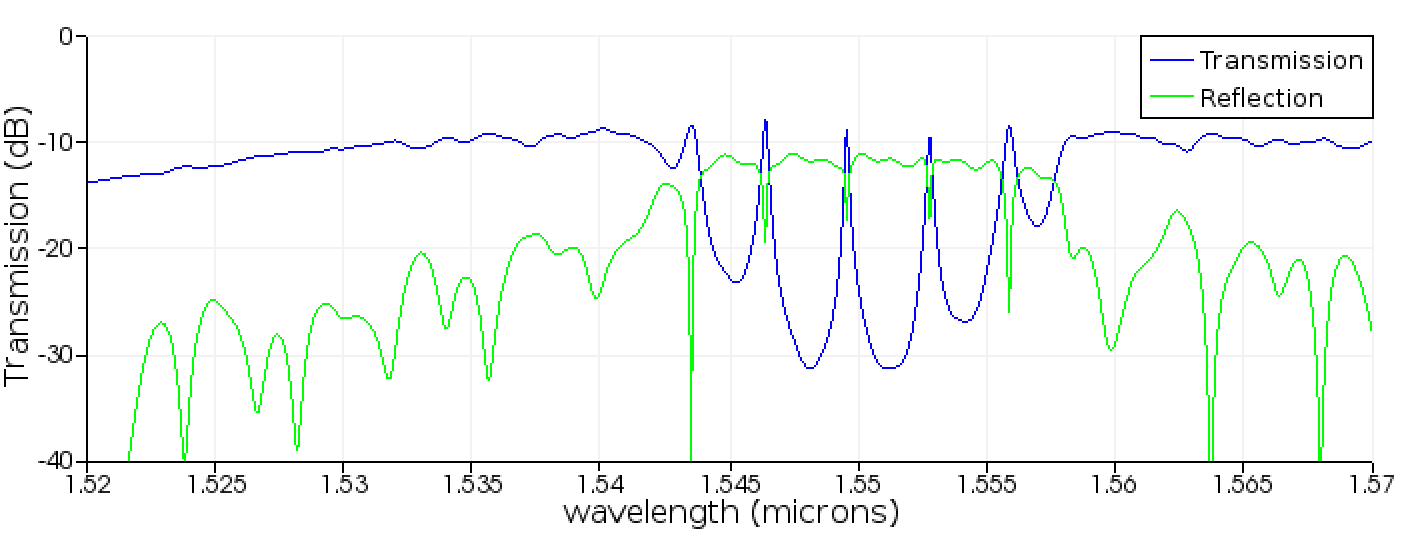
\includegraphics[width=0.8\linewidth]{../figs_paper/Bragg} }
\caption{Layout and simulations of a Bragg grating cavity.}
\label{Bragg}
\end{center}
\end{figure}



\graphicspath{{../figs_chris/}}

\begin{figure}[tbp]
	\centering
	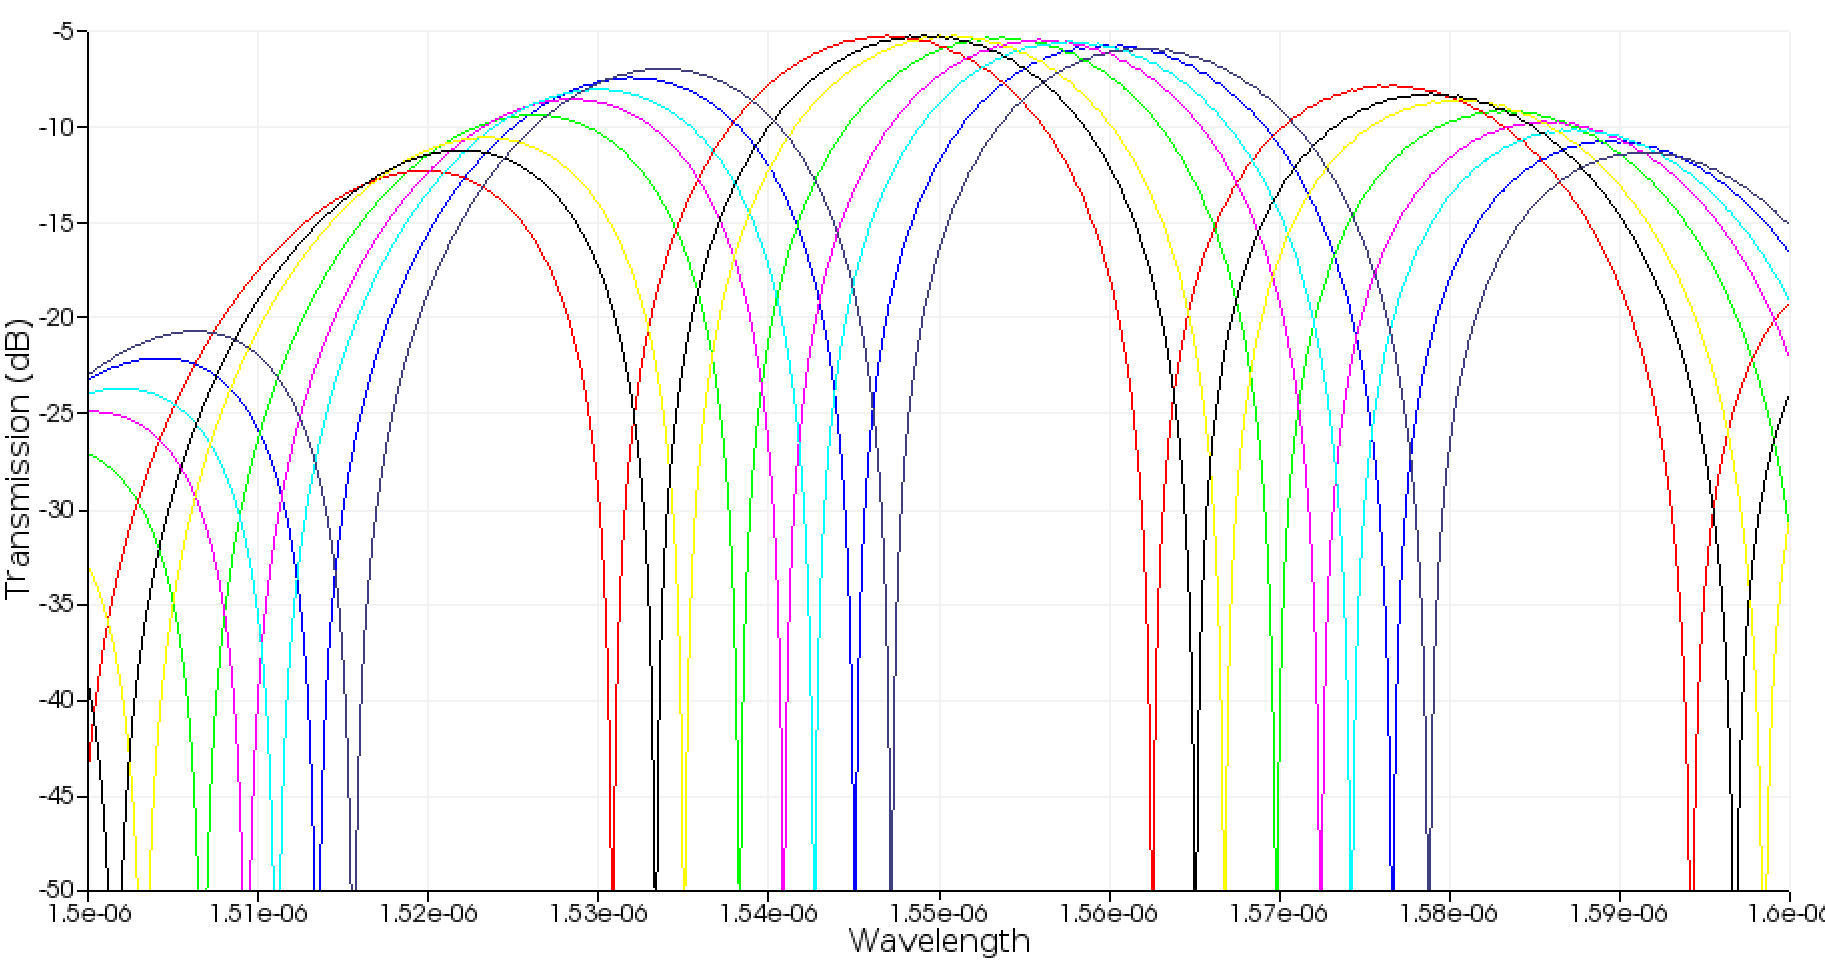
\includegraphics[width=0.8\textwidth]{../figs_paper/MZI_circuit2_MC.png}
    \caption[]{Monte Carlo simulation of the Mach-Zehnder Interferometer layout in Figure~\ref{MZI_circuit2}.}
    \label{MZI_circuit2_MC}
\end{figure}



%%%%%%%%%%%%%%%%%%%%%%%%%%%%%%%%%%%%%%%%%%%%%%%%%%%%%%%%%%%%%%%%%%%%%%
\section{Manufacturing Variability}
\label{sec:variability}
The high refractive index contrast of SOI permits sharp waveguide bends and ultra-small device sizes, making it promising for the development of densely integrated photonic circuits. However, silicon photonic devices face serious manufacturability challenges. Fabrication errors on either the waveguide width or waveguide thickness have a significant effect on the propagation constant of light, and, thus, circuits such as interferometers are highly sensitive to manufacturing, as shown in Figure~\ref{MZI_circuit2_MC}.

Thus, taking manufacturing variability into account in order to predict yield is critical for photonic integrated circuits. In the electronics community, corner analysis and Monte Carlo simulations are typically used to analyze fabrication variability; the former of predicts the worst-case performance of the circuit, while the later creates histograms and distributions, and is typically based on process variations applied to the entire circuit.  In the simplest Monte Carlo approach, the same variations are applied to all components in the circuit, thus the simulation considers common-mode variability only (i.e., all devices are slightly thicker).  

\subsection{Component models taking into account variability}
In order to perform Monte Carlo simulations, we require parameterized component models that are continuous with the variables of interest (e.g., thickness, width).  Although one approach is to simulate each component on a fine mesh (e.g., 0.1 nm steps in each deviation variable), this may be computationally prohibitive.  We developed more efficient approaches, as follows.

\subsubsection{S-Parameter component models}
A multidimensional spline interpolation method allows for estimation of the amplitude and phase for each S-parameter taking into account its dependency on multiple parameters, such as frequency, thickness and width. S-parameters passivity and reciprocity can also be tested and enforced, to avoid violating energy conservation laws.

For components that are described by S-parameters, we begin by generating S-parameters for the corner cases (e.g., components with variations ($\Delta$w (nm), $\Delta$h (nm)) of (+20, +10), (+20, -10), (-20, +10) and (-20, -10)), as shown in Fig.~\ref{s-interpolation}(a).  For each Monte Carlo iteration, we interpolate the S-parameters for the desired thickness and width variation. The model can include multiple modes (e.g., TE and TM polarization).

This can be applied to components such as directional couplers, where the phase through the device is dependant on the thickness and width of the waveguide.  Two directional couplers can be connected to create a ring resonator sub-circuit, and the performance of the ring resonator (resonance frequency, free spectral range, extinction ratio) will vary with the thickness and width variability introduced into the directional coupler model. As an example, Fig.~\ref{s-interpolation}(b) shows the S-parameters for both the corner and interpolated cases of a 2$\times$2 power splitter.






\begin{figure}[tbp]
	\centering
	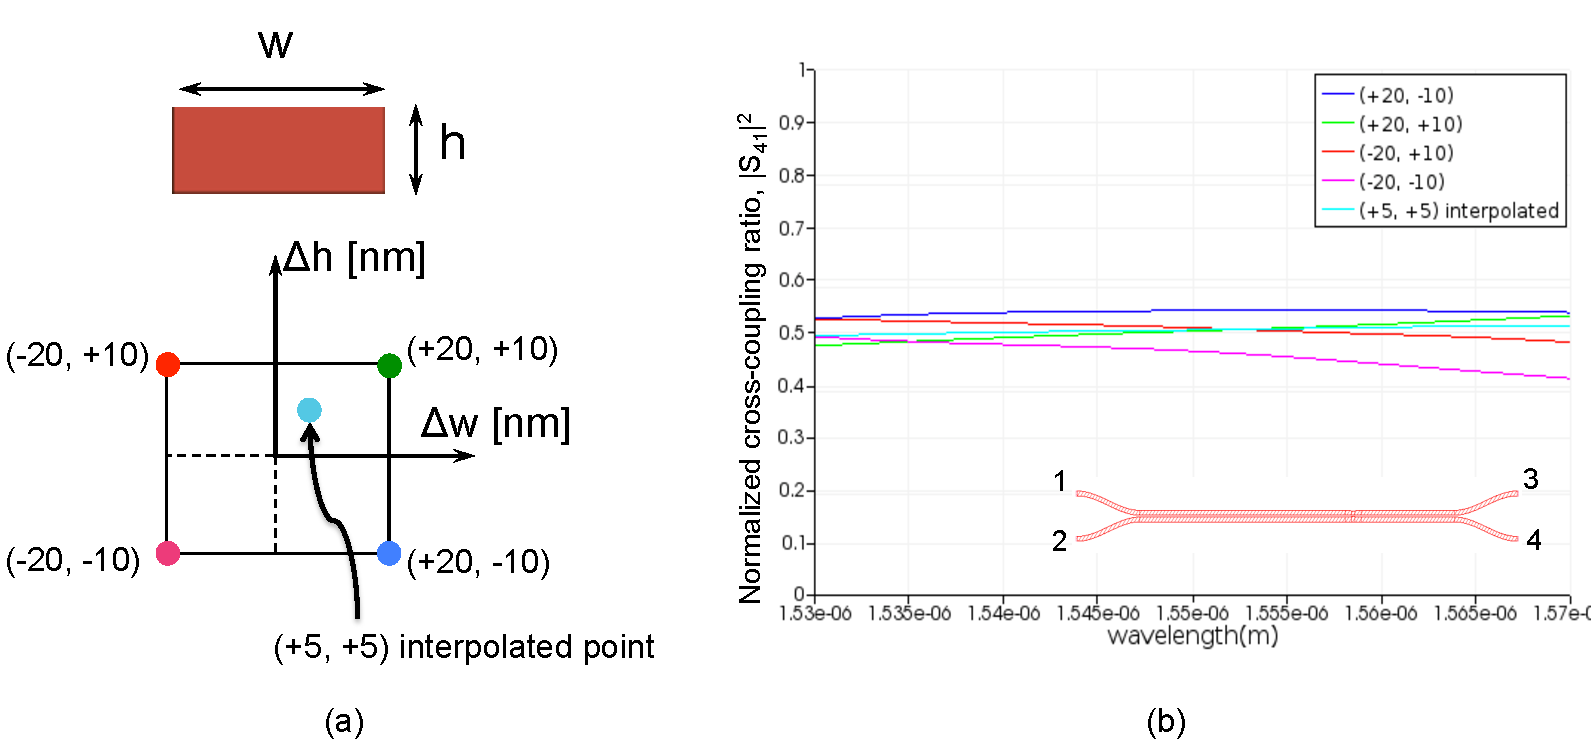
\includegraphics[width=0.8\textwidth]{../figs_paper/S_Interpolation.pdf}
    \caption[]{(a) Process corners for two process parameters: waveguide height and width; (b) S-parameter interpolation for a 2$\times$2 power splitter.}
    \label{s-interpolation}
\end{figure}

\begin{figure}[tbp]
	\centering
	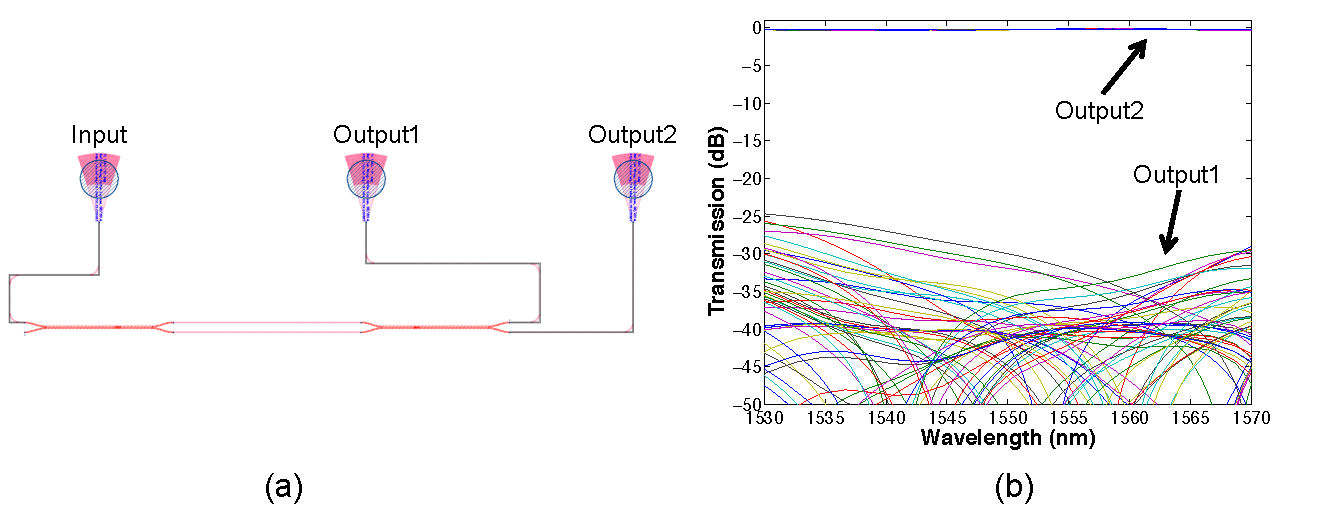
\includegraphics[width=0.8\textwidth]{../figs_paper/MZI_common_MC.pdf}
    \caption[]{(a) Layout of balanced Mach-Zehnder Interferometer test structure; (b) Monte Carlo simulation results for the output transmissions.}
    \label{MZI_commmon_MC}
\end{figure}

\subsubsection{Waveguides}
2D case. easiest is to simply parameterize the effective index as a function of the thickness and width.

*****  add something intelligent here *****
The waveguide transfer function is described by propagation properties such as loss, effective index, group index and dispersion, and are parameterized as a function of frequency, thickness and width. 

\subsubsection{Perturbation approach}
For the case of the Bragg grating, for example, we can assume that the manufacturing only affects the central Bragg wavelength.  If all other parameters remain the same (grating coupling coefficient) than a small perturbation to the nominal effective index can be applied.  This can be expressed as two independent linear parameters, $ \frac{\partial n_\text{eff}}{\partial w}$, and $ \frac{\partial n_\text{eff}}{\partial h}$, which are added to the nominal value.

\subsection{Uniform Monte Carlo}
***please add text for Figure~\ref{MZI_commmon_MC}*** 

\subsection{Enhanced Monte Carlo}

The challenge in these simulations is to capture the die-to-die, device-to-device, and intra-device variations, which have position-dependant correlations.  Correlated yield analysis is attracting increasing attention, and there have been studies investigating the statistical on-chip correlations \cite{lukas14:OFC,hochberg:wafer}, and models for dealing with the uncertainty of devices \cite{MIT:uncertainty}.  From this past work, what is clear is if only common-mode variability is considered (corner analysis, Monte Carlo described above), the simulations do not capture an important type variability -- differential.  Namely, two nominally identical devices side-by-side on a chip will have slightly difference performance.  This difference can have significant impact on system performance (e.g., WDM ring resonators, optical switches) and it cannot be simply compensated by thermally tuning the entire chip.

In this work, we propose, for the first time, a methodology that takes correlation between devices into account by using the physical layout in order to perform a manufacturing variability analysis of on-chip photonic integrated circuits. Beginning with the physical layout, and performing to enhanced Monte Carlo simulations, our methodology  provides insight into the significance of compact layouts for photonic designs, and offers a useful tool for post-layout verification and power trimming estimation.

\begin{figure}[h]
    \centering
    \label{flow_chart}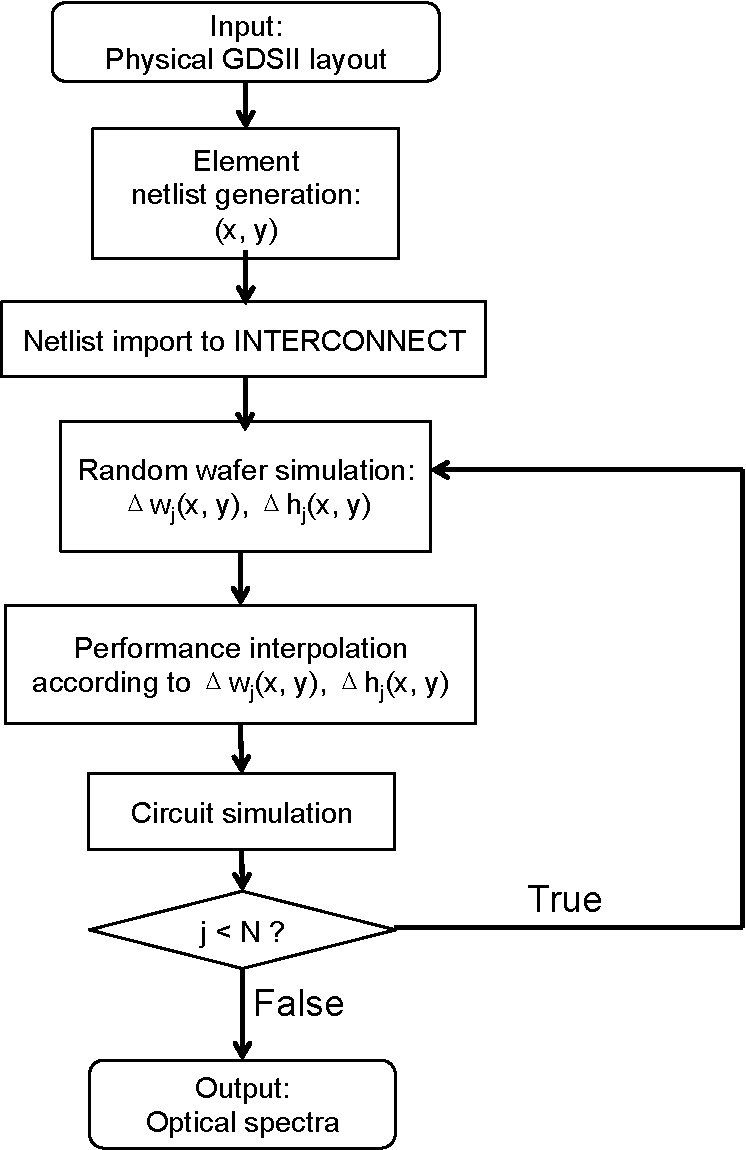
\includegraphics[width=\linewidth]{flow_chart.pdf}
    \caption{(a) Flow chart of the proposed methodology; (b) simulated waveguide linewidth deviations across a wafer; (c) simulated waveguide thickness deviations across a wafer.}
    \label{flow_chart}  
\end{figure}

Figure \ref{flow_chart}(a) shows the flow chart of our proposed methodology. The procedure includes: 
\begin{itemize}
\item First, the layout for silicon photonic circuits and/or devices under test are created.  In the example presented here, they are designed using KLayout \cite{www_klayout}. 
\item
The netlist is extracted from the layout, either using Mentor Graphics LVS or the SiEPIC-EBeam-PDK add-on \cite{siepic-ebeam-pdk} to KLayout \cite{www_klayout}.  The netlist provides a list of the primitive components in the library and the connectivity between components.  The netlist is imported into Lumerical INTERCONNECT for circuit simulations. 
\item
The third step is a wafer simulation.  In INTERCONNECT, silicon waveguide width deviations, $\Delta w(x,y)$, and wafer thickness deviations, $\Delta h(x,y)$, are simulated across the whole wafer, as illustrated in the maps in Figures~\ref{flow_chart}(b) and \ref{flow_chart}(c), respectively. Both deviations are characterized by a sigma RMS amplitude and a correlation length, and both are based on experimental results \cite{lukas14:OFC,hochberg:wafer}. In each run of the Monte Carlo simulation, different deviation maps are be generated. 
\item
According to the spatially-dependent waveguide width and thickness deviations, the optical S-parameters of primitive elements and the optical propagation constants of connecting waveguides are calculated.  This is performed using interpolation in INTERCONNECT. 
\item
The circuit with components updated based on their position is simulated.  This is repeated several times, and the results can be visualized, as in Figure~\ref{MZI_circuit2_MC}. Histograms and statistical analysis can be performed, as in Figure~\ref{error}.
\end{itemize}

\begin{figure}[t]
    \centering
    \label{error}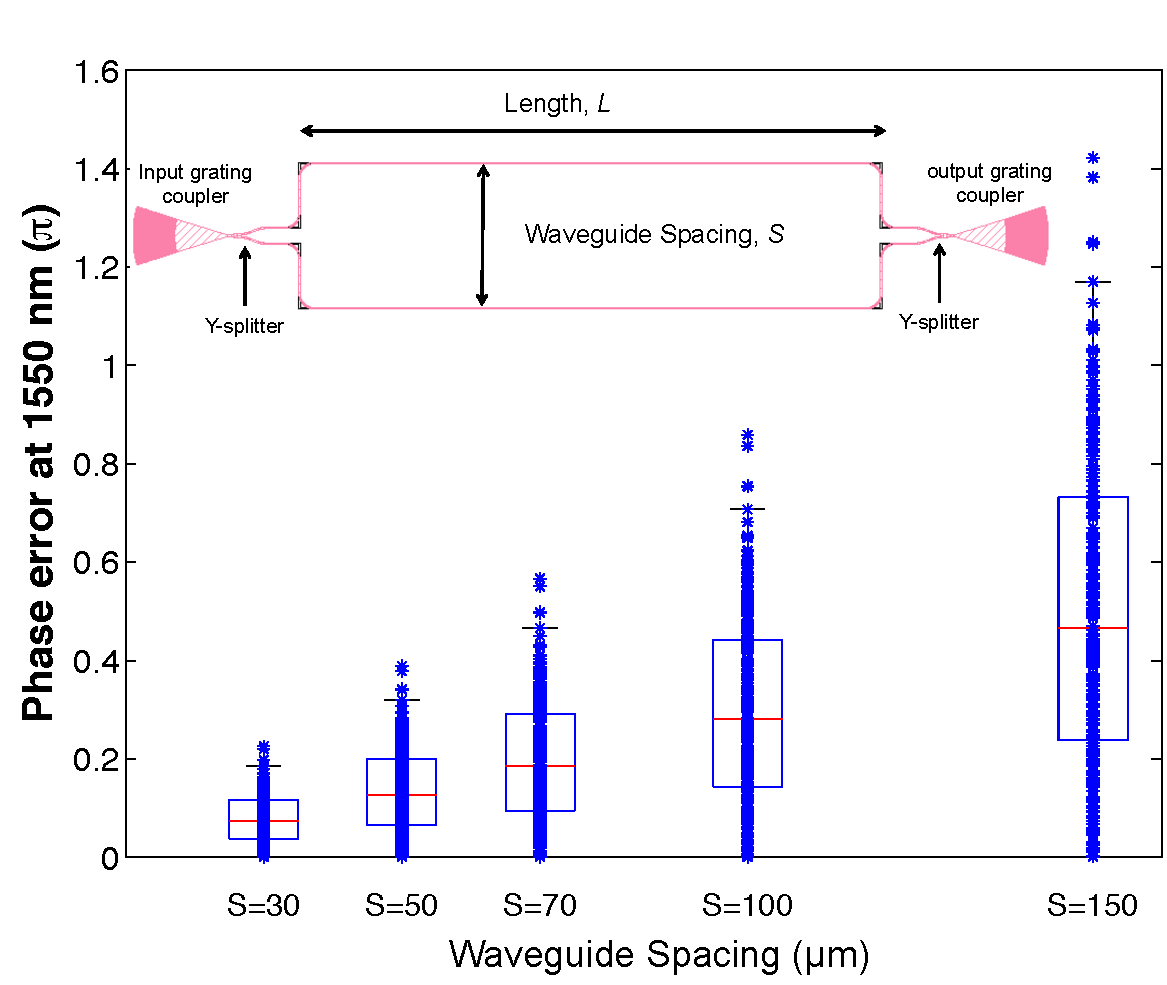
\includegraphics[width=0.8\linewidth]{error.pdf}
    \caption{Box scatter plot of the phase error of a balanced Mach-Zehnder Interferometer versus waveguide spacing, generated using the Enhanced Monte Carlo simulations.} 
    \label{error}
\end{figure}


The scatter plot in Figure~\ref{error} shows the simulated phase error of a balanced Mach-Zehnder Interferometer versus the waveguide spacing between two arms, in a 248 nm silicon photonics process. In the Monte Carlo simulations, the horizontal length of the phase arms, $L$,  is 200 $\mu m$. The phase error is defined as the absolute optical phase difference between the two phase arms. Ideally, the phase error should be 0 when there are no fabrication variations. However, this figure clearly shows that the mean of the phase error for an ensemble of MZIs is approximately linearly proportional to the waveguide spacing, emphasizing the importance of very compact layout designs, particularly where phase matching is required.  This simulation is similar to the proportionality  observed experimentally in ring resonators \cite{lukas14:OFC}.  The simulated phase error can be used to estimate the trimming power required for MZI-based photonic switches. 



\section{Conclusion}\label{sec6}

%The opportunity for silicon photonics is to leverage three decades of CMOS Electronic Design Automation (EDA) tool development, and two decades of optical design software development.
%Full-flow design environments are becoming a reality for silicon photonics.
%
%The mature CMOS fabrication processes and multi-project wafer (MPW) fabrication runs 
%%Stable processes that are repeatable
%enable the development of component libraries for system design.  Emphasis needs to be placed on developing parameterized components to bring increased utility for system-level design, and incorporating manufacturing yield and process variations into the design flow.  
%
%Similar to the electronics industry, photonic integrated circuit design and fabrication is evolving towards specialized roles, namely: a) fabrication and processing, b) EDA tools; c) component, library, and PDKs; and, d) system design.  This separation of roles will lead to accelerated product development and ultimately aiding the silicon photonics industry achieve its objectives. 


The  objective of this work is ``first-time-right'' design, where circuits function correctly the first time they are fabricated; this can be achieved only if the designer takes manufacturing challenges into consideration and applies effective mitigation strategies in order to build circuits that are immune to these variations.



\acknowledgments

The authors would like to thank CMC Microsystems for enabling the fabrication of numerous chips via imec-ePIXfab and IME.  Funding for this research was provided by NSERC, particularly the NSERC CREATE Silicon Electronic Photonic Integrated Circuits (SiEPIC) training program, \url{http://www.siepic.ubc.ca}.
%The authors are grateful to Nicolas A.F.~Jaeger and Tom Baehr-Jones for useful discussions. 

\bibliography{../Refs/references}
\bibliographystyle{spiebib33}


\end{document}
